% Original anatomical pixels retained; schematic connections are conceptual.
\documentclass[tikz,border=3pt]{standalone}
\usepackage[T1]{fontenc}
\usepackage{graphicx}
\usetikzlibrary{arrows.meta,positioning}
\definecolor{ink}{HTML}{233747}
\definecolor{blue}{HTML}{256B91}
\definecolor{rust}{HTML}{B95020}
\begin{document}
\begin{tikzpicture}[x=1cm,y=1cm,
 every node/.style={font=\sffamily\fontsize{9}{11}\selectfont,text=ink,align=center},
 box/.style={draw=blue!45,fill=blue!5,rounded corners=4pt,minimum height=1.15cm,text width=3.4cm,inner sep=6pt},
 arrow/.style={-{Stealth[length=5pt]},line width=.9pt,draw=rust},
 head/.style={font=\sffamily\bfseries\fontsize{11}{13}\selectfont,text=blue}]
\path[use as bounding box] (0,0) rectangle (18,9.1);
\node[head,anchor=west,text=rust] at (.15,8.8) {From fly anatomy to hexapod control};
\draw[rounded corners=5pt,draw=blue!30,fill=blue!4] (0,.85) rectangle (5.25,8.3);
\node[head] at (2.63,7.95) {Anatomical reference};
\node at (1.8,4.63) {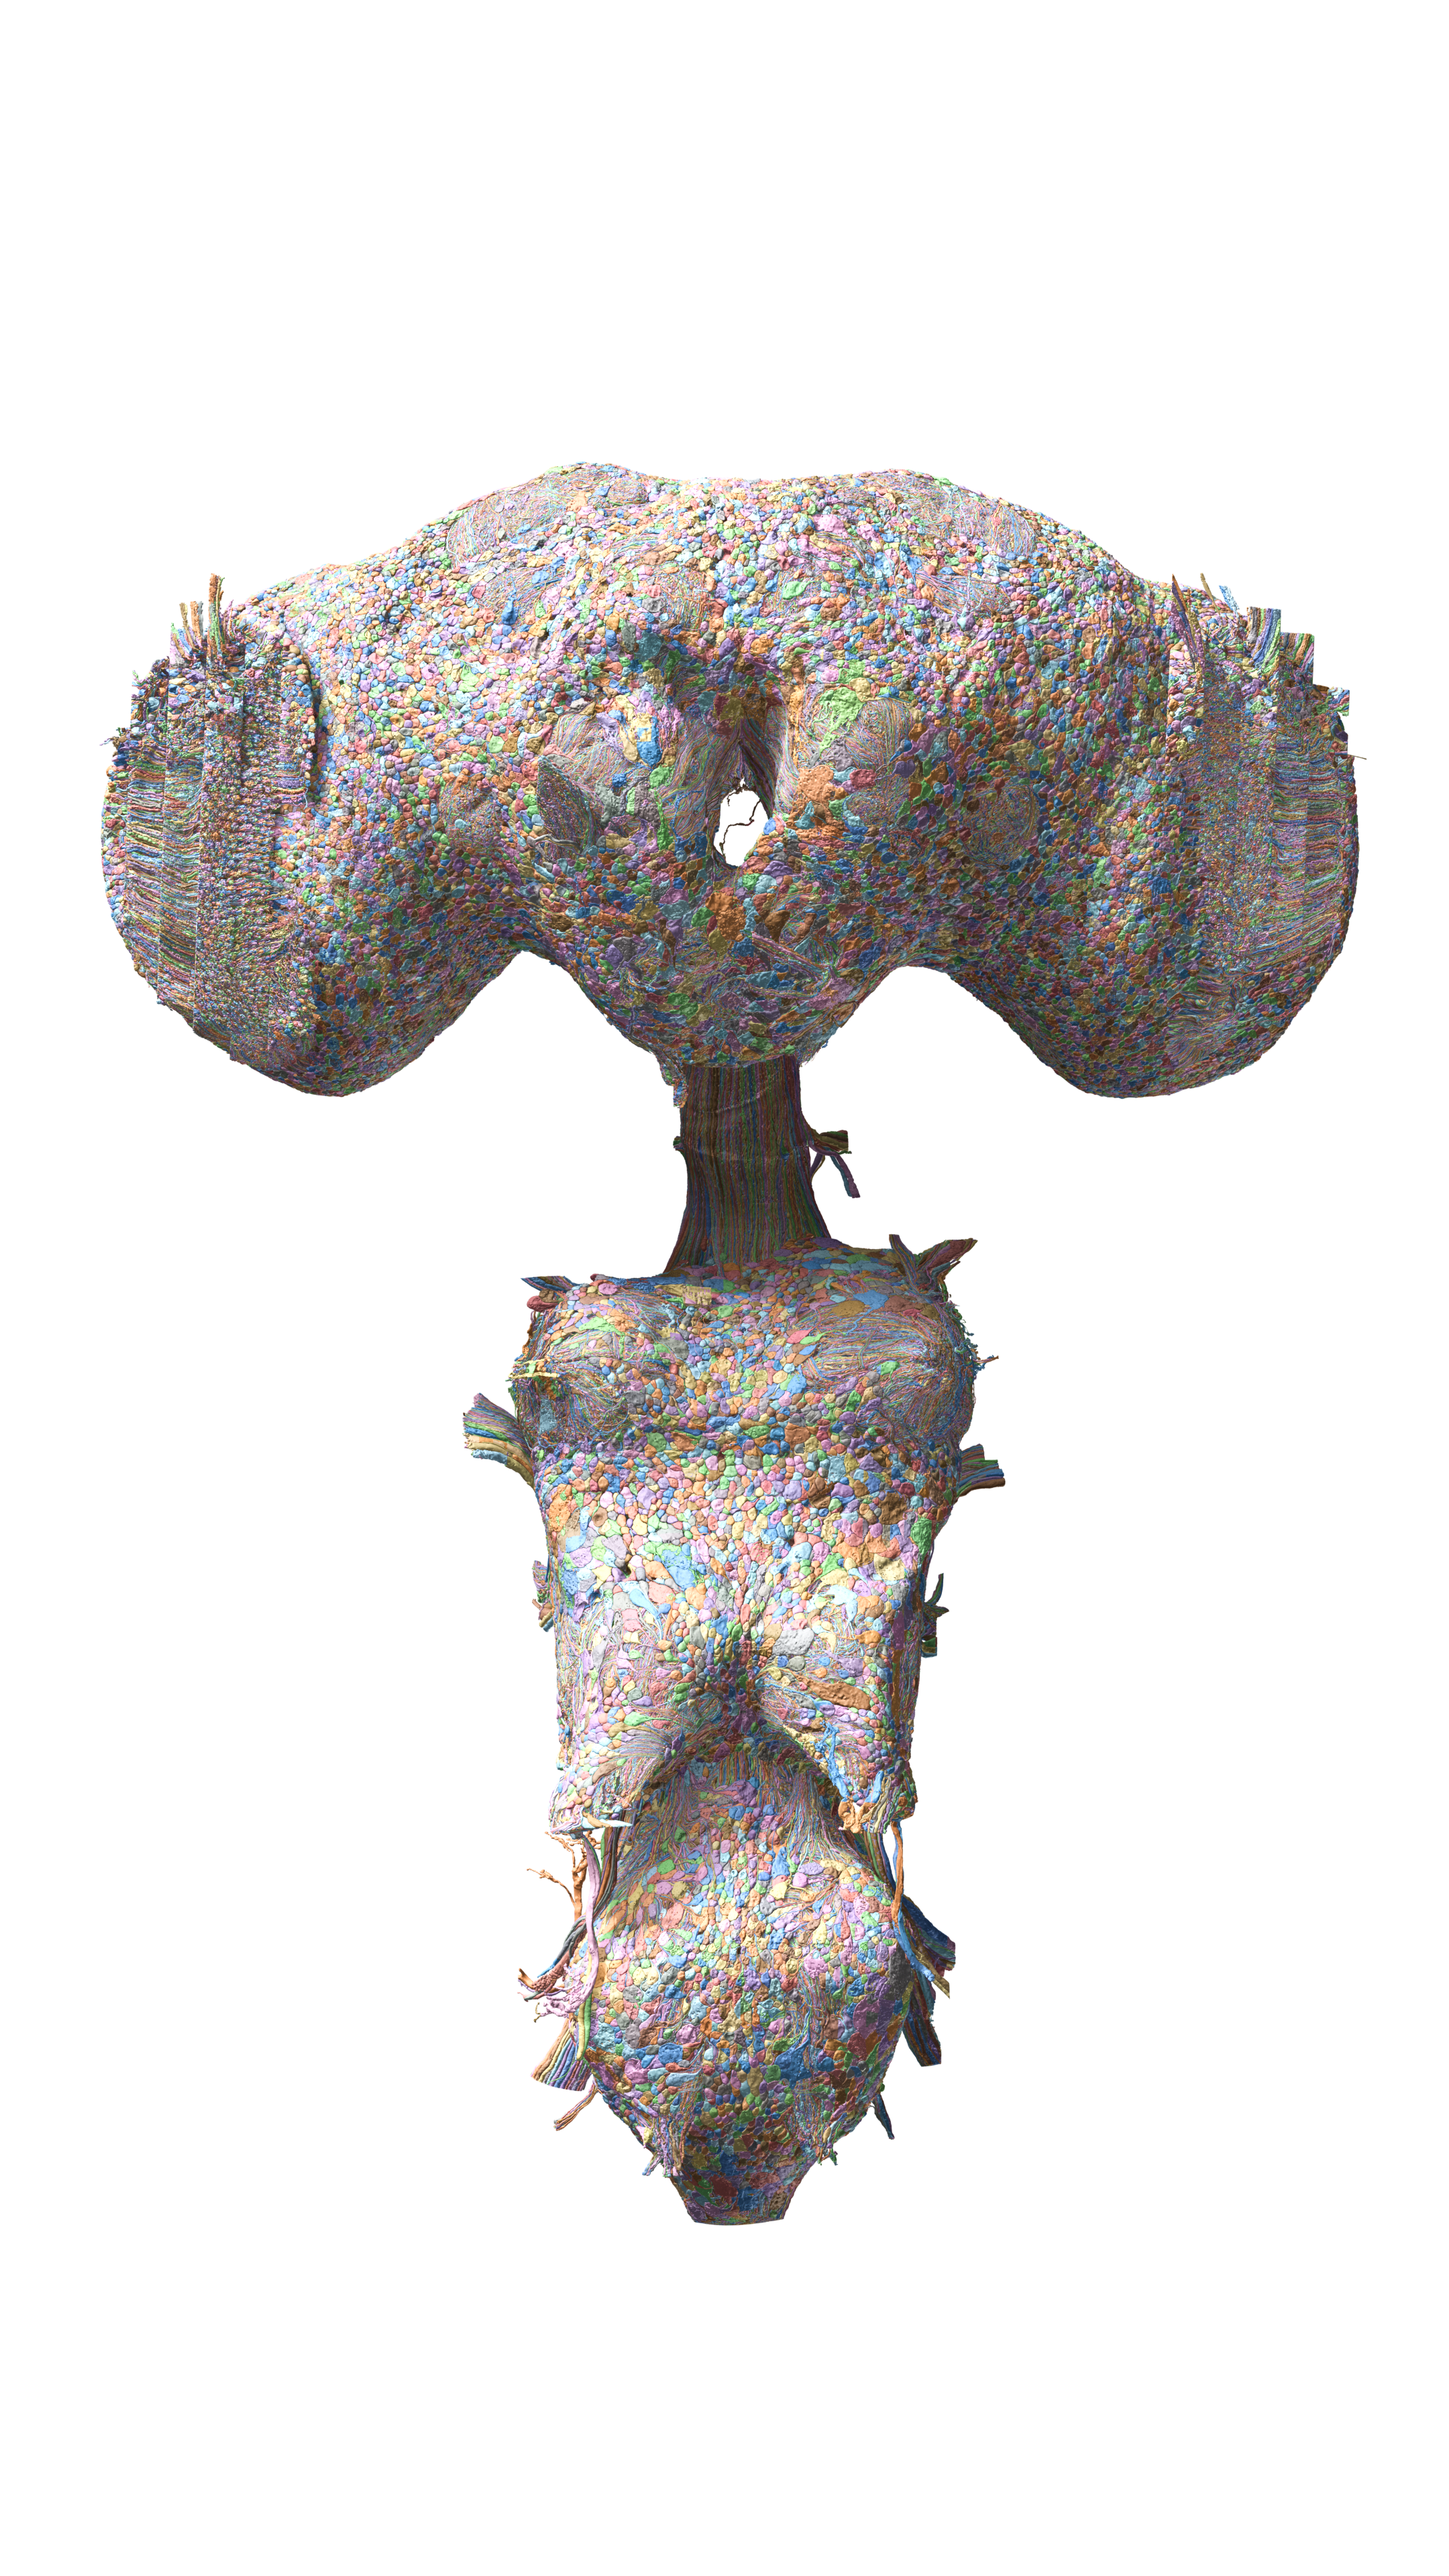
\includegraphics[height=5.15cm,trim=120 470 100 640,clip]{fly_brain_vnc.png}};
\node[anchor=west] (brain) at (3.85,6.8) {Brain};
\draw[arrow] (brain.west) -- (2.9,6.65);
\node[anchor=west,text=rust] (vnc) at (3.55,3.7) {VNC};
\draw[arrow] (vnc.west) -- (2.5,3.7);
\node[text width=4.6cm,font=\sffamily\fontsize{8}{10}\selectfont] at (2.63,1.45)
 {Brain shown for context.\\The model uses a selected VNC-centered network.};

\node[head] at (9.3,7.95) {Fixed network and motor map};
\node[box] (input) at (9.3,6.85) {\mbox{Named descending}\\inputs\\\textbf{External Poisson drive}};
\node[box] (core) at (9.3,5.2) {\textbf{Frozen VNC model}\\11,000 nodes; 485,074 edges};
\node[box] (map) at (9.3,2.9) {\textbf{260 motor channels}\\Opposing pool means\\$\downarrow$\\Fixed gains and joint grouping};
\draw[arrow] (input) -- (core);
\draw[arrow] (core) -- node[right,font=\sffamily\fontsize{8}{10}\selectfont] {Motor rates} (map);
\draw[arrow,dashed] (5.25,4.6) -- node[above,text width=1.65cm,font=\sffamily\fontsize{8}{10}\selectfont] {Measured\\wiring} (core.west);

\node[head] at (15.25,7.95) {Simulated body};
\node at (15.25,5.95) {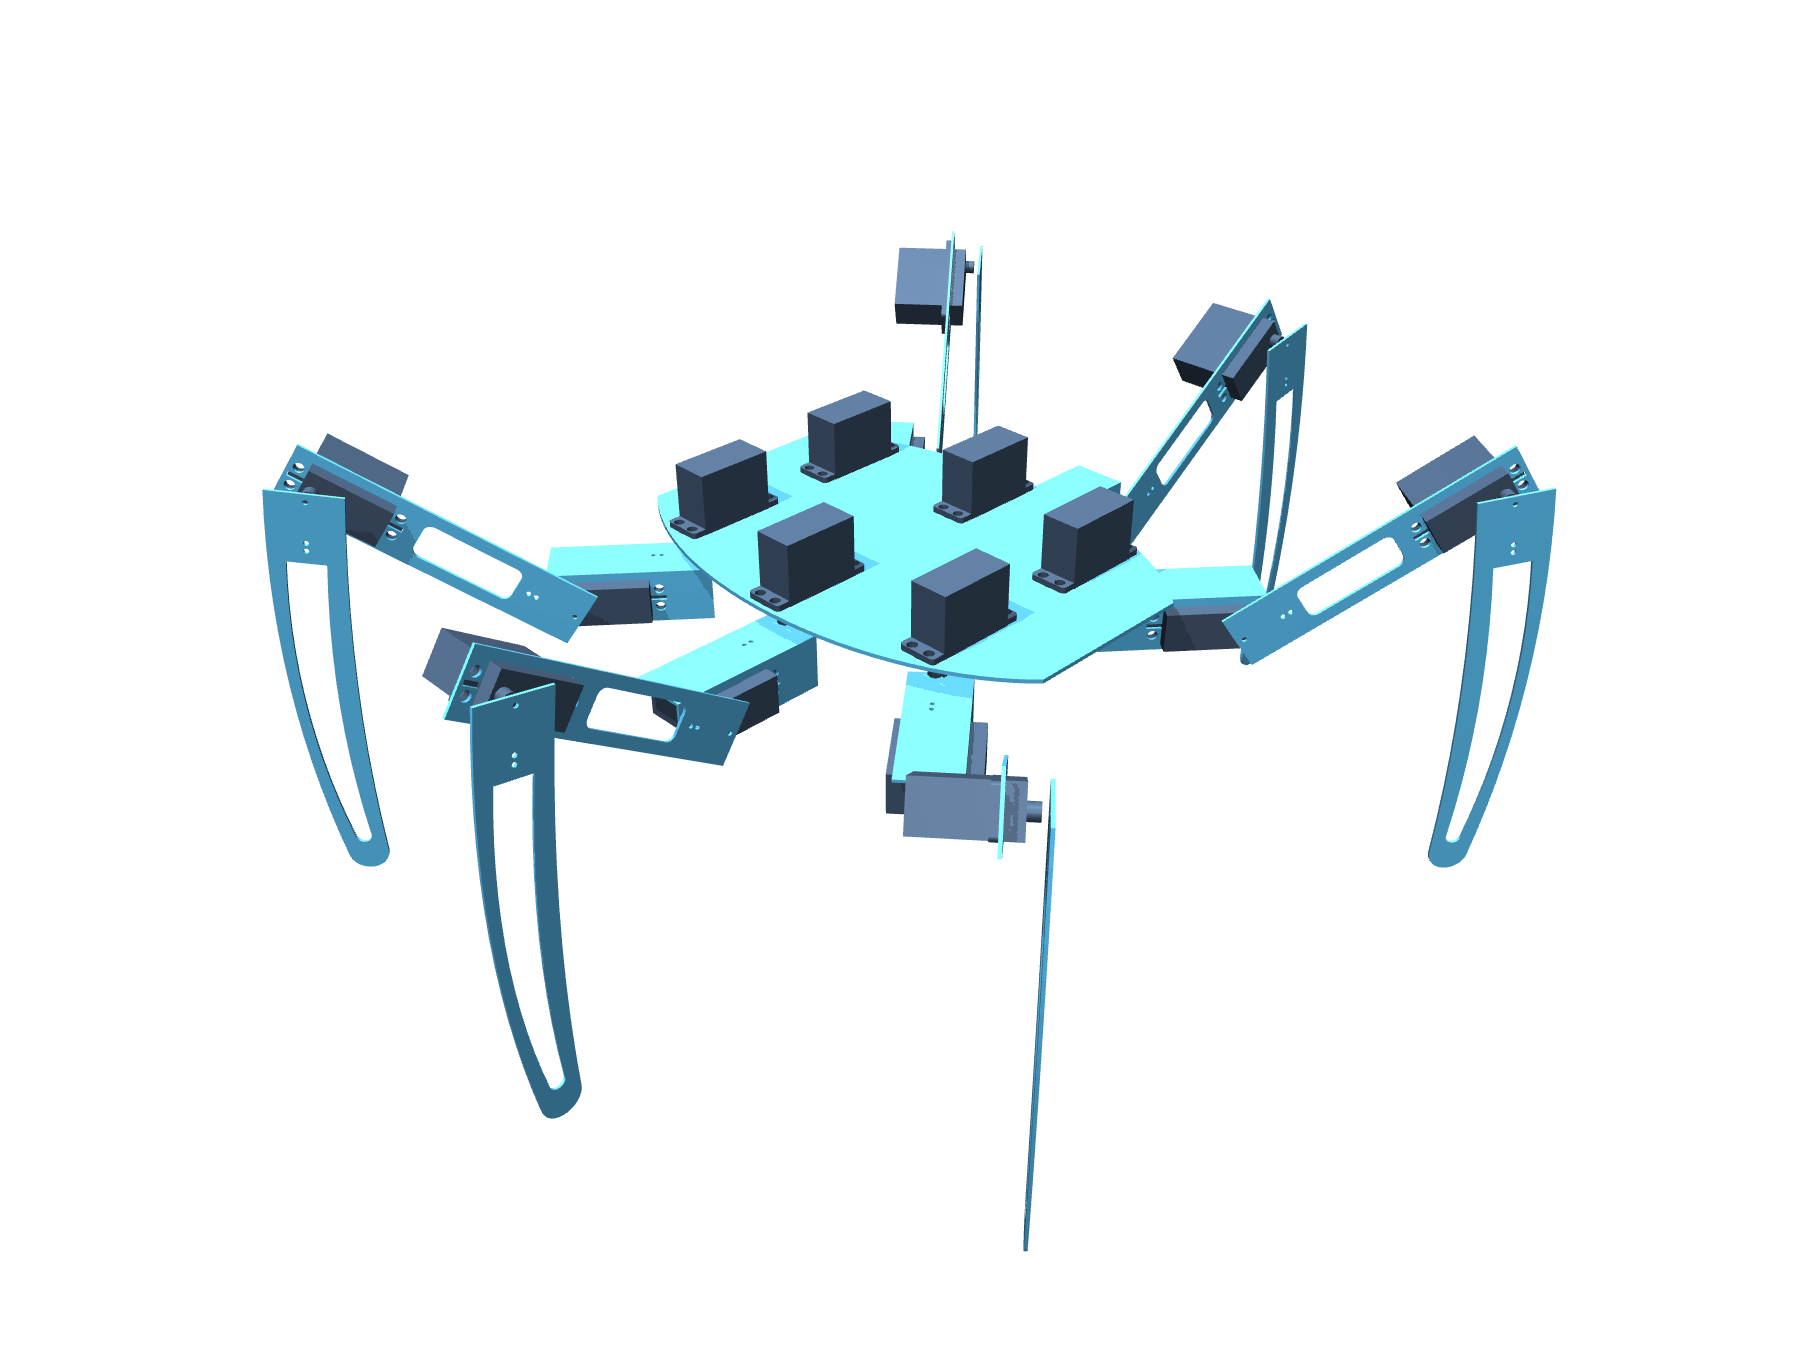
\includegraphics[width=4.7cm,trim=200 60 200 200,clip]{hexapod_model.png}};
\node[box,text width=3.6cm] (body) at (15.25,2.9) {\textbf{18 joint targets}\\PD joint controller\\6 legs in MuJoCo};
\draw[arrow] (map.east) -- node[above,text width=1.9cm,font=\sffamily\fontsize{8}{10}\selectfont] {Target\\angles} (body.west);
\draw[arrow] (body.north) -- (15.25,4.4);
\node[text width=10.9cm,font=\sffamily\fontsize{8}{10}\selectfont] at (12.0,1.15)
 {Fixed-map experiment: no learned conversion and no body feedback to the network.\\Walking experiments add a separate rhythm generator, not shown here.};
\node[anchor=west,font=\sffamily\fontsize{7}{9}\selectfont,text=ink!75] at (.1,.3)
 {Anatomy: MaleCNS / Janelia FlyEM and collaborators, CC BY 4.0. Schematic, not to scale.};
\end{tikzpicture}
\end{document}
